\section{Experiments}
\label{sec:experiments}

Every number in this section is produced by \texttt{scripts/make\_paper\_tables.py} from the released result files;
the tables are included verbatim. Arena and continuous-turn results are over \nSeeds\ seeds, NYC over \nSeedsNyc.

\subsection{Prediction accuracy is not what the wiring buys}
\label{sec:prediction}

\begin{table*}[t]
  \centering\small
  \setlength{\tabcolsep}{4pt}
  \begin{tabular}{lcccccc}
    \toprule
    & \multicolumn{2}{c}{Arena (5 seeds)} & \multicolumn{2}{c}{Cont.\ turns (0 seeds)} & \multicolumn{2}{c}{NYC twin (3 seeds)} \\
    \cmidrule(lr){2-3}\cmidrule(lr){4-5}\cmidrule(lr){6-7}
    wiring & MSE $\downarrow$ & cos $\uparrow$ & MSE $\downarrow$ & cos $\uparrow$ & MSE $\downarrow$ & cos $\uparrow$ \\
    \midrule
    GRU, parameter-matched & \textbf{0.434\pm0.004} & \textbf{0.72} & -- & -- & \textbf{0.609\pm0.003} & \textbf{0.56} \\
    GRU, recurrent-budget-matched & 0.501\pm0.001 & 0.67 & -- & -- & -- & -- \\
    dense & 0.562\pm0.004 & 0.63 & -- & -- & -- & -- \\
    connectome, unsigned & 0.573\pm0.001 & 0.63 & -- & -- & -- & -- \\
    connectome, random signs & 0.578\pm0.001 & 0.62 & -- & -- & -- & -- \\
    \textbf{connectome} & 0.579\pm0.003 & 0.62 & -- & -- & 0.701\pm0.010 & 0.47 \\
    random & 0.583\pm0.002 & 0.61 & -- & -- & 0.707\pm0.007 & 0.48 \\
    block-shuffled & 0.585\pm0.005 & 0.61 & -- & -- & 0.726\pm0.014 & 0.45 \\
    degree-shuffled & 0.610\pm0.002 & 0.59 & -- & -- & 0.731\pm0.005 & 0.45 \\
    \midrule
    copy last visible latent & 0.811 & -- & -- & -- & 1.558 & -- \\
    constant mean & 0.992 & -- & -- & -- & 0.977 & -- \\
    \bottomrule
\end{tabular}

  \caption{\textbf{Blind-horizon latent prediction.} Mean MSE over blind horizons 1 to 8 in whitened PCA-256 space
  (mean\pm sd over seeds) and cosine to the teacher latent, on the arena, on the arena with continuous turn angles and
  on the NYC twin. Every student beats both trivial predictors. The parameter-matched GRU and transformer beat every
  sparse student; among sparse wirings of identical size the real connectome is the best by about one percent. The
  attention-input rows replace the shared linear input map by a per-neuron cross-attention encoder (\cref{sec:student});
  the hybrid row adds one attention layer over cell-type tokens to the connectome recurrence.}
  \label{tab:pred}
\end{table*}

\cref{tab:pred} gives the headline prediction numbers. Every student is far below both trivial predictors. Among sparse
wirings of identical size the real connectome is the best, by \nConnOverBlockArena\,\% of latent error over
block-shuffled, and the margin is reproducible: it holds on every seed, on the continuous-turn data, on the NYC twin, at
every training-set size from 50 to 500 episodes (\cref{sec:suppl-data}) and on every subgraph we ablate
(\cref{sec:ablation}). But it is small, and the dense sequence models are clearly better: the parameter-matched GRU by
\nGruBetterArena\,\%, the parameter-matched transformer by \nTfBetterArena\,\% (\nGruBetterNyc\ and \nTfBetterNyc\,\% on
NYC). Sign structure does not help prediction either: the unsigned student is marginally better than the signed one.
We therefore make no claim that the connectome is a better predictor. It is a worse one, and what follows is about what
it does instead.

\subsection{The connectome state path-integrates in the dark}
\label{sec:probes}

\begin{table*}[t]
  \centering\small
  \setlength{\tabcolsep}{3.5pt}
  \begin{tabular}{lcccccc}
    \toprule
    & \multicolumn{2}{c}{Arena} & \multicolumn{2}{c}{Continuous turns} & \multicolumn{2}{c}{NYC twin} \\
    \cmidrule(lr){2-3}\cmidrule(lr){4-5}\cmidrule(lr){6-7}
    wiring & heading err & pos $R^2$ & heading err & pos $R^2$ & heading err & pos $R^2$ \\
    \midrule
    GRU, parameter-matched & 30.6\pm0.6 & 0.41\pm0.01 & -- & -- & 45.4\pm2.6 & 0.25\pm0.01 \\
    GRU, recurrent-budget-matched & 35.5\pm0.7 & 0.30\pm0.01 & -- & -- & -- & -- \\
    dense & 21.3\pm0.7 & 0.68\pm0.01 & -- & -- & -- & -- \\
    connectome, unsigned & 13.8\pm0.8 & 0.88\pm0.01 & -- & -- & -- & -- \\
    connectome, random signs & 9.2\pm1.3 & \textbf{0.94\pm0.01} & -- & -- & -- & -- \\
    \textbf{connectome} & \textbf{9.1\pm1.2} & 0.94\pm0.01 & -- & -- & \textbf{9.4\pm0.7} & \textbf{0.94\pm0.01} \\
    random & 12.9\pm0.7 & 0.88\pm0.01 & -- & -- & 15.1\pm0.7 & 0.89\pm0.00 \\
    block-shuffled & 10.8\pm0.8 & 0.93\pm0.01 & -- & -- & 10.1\pm1.1 & 0.94\pm0.02 \\
    degree-shuffled & 12.7\pm0.6 & 0.89\pm0.02 & -- & -- & 14.3\pm2.0 & 0.84\pm0.01 \\
    \midrule
    actions only (linear floor) & 40.1 & 0.54 & -- & -- & 22.6 & 0.41 \\
    integrator of the action record & 0.0 & 1.00 & -- & -- & 0.0 & 1.00 \\
    \bottomrule
\end{tabular}

  \caption{\textbf{Heading and position decoded from the state during 8 blind steps.} Ridge probe; median absolute
  heading error in degrees and position $R^2$ relative to the start of the window, mean\pm sd over seeds. With
  continuous turn angles the action record no longer determines heading, so the integrator row is no longer exact and
  the probe measures integration of a noisy signal. The connectome keeps a linearly readable heading and position code
  that neither the GRU nor the transformer forms; sparse controls of the same size form a slightly worse one.}
  \label{tab:probe}
\end{table*}

\cref{tab:probe} and \cref{fig:main} are the main result. During the 8 blind steps the connectome state carries heading
to \nConnArenaHd\degree\ median error and position to $R^2$\,\nConnArenaPos\ on the arena, \nConnNycHd\degree\ and
\nConnNycPos\ on NYC. The parameter-matched GRU, which predicts the teacher far better, gives \nGruArenaHd\degree\ and
\nGruArenaPos\ on the arena; the transformer, which also predicts better and can attend over its whole visible past,
gives \nTfArenaHd\degree\ and \nTfArenaPos. Three controls fix what this does and does not mean.

\paragraph{Information ceiling} With fixed-angle turns and actions given in the dark, a closed-form integrator of the
action record recovers heading exactly, so on the arena the probe does not ask whether heading \emph{can} be known; it
asks whether the state \emph{keeps} it in a population code a linear readout can use. A linear probe on the cumulative
action counts alone reaches \nActOnlyArenaHd\degree\ (a linearity floor, not an information floor). The continuous-turn
columns remove the ceiling: every turn is scaled by a $\mathcal{N}(1, 0.3)$ factor, the integrator of the discrete record
is wrong by \nIntegratorTnHd\degree\ on median, and the connectome state decodes to \nConnTnHd\degree. Whatever it
integrates there is not the action record.

\paragraph{Non-linearity} \cref{tab:dark} repeats the probe with an MLP. An MLP on the GRU state gives
\nGruArenaMlpHd\degree, so the GRU is not hiding the code non-linearly; on the sparse students the same probe
\emph{improves} heading to \nConnArenaMlpHd\degree\ (connectome) and \nBlockArenaMlpHd\degree\ (block-shuffled). The
gap widens under the non-linear probe.

\paragraph{Feature count} A random 762-neuron subset of the connectome (the GRU's width) decodes heading at
19\degree, still better than the full GRU state (\cref{sec:suppl-probe}).

\paragraph{What the wiring contributes} Sign structure matters, but not which signs: the unsigned student loses the
code (\nNosignArenaHd\degree, $R^2$\,\nNosignArenaPos) while random Dale-consistent signs match the real ones. The exact
synapse list matters a little: the real wiring beats block-shuffled by \nConnBlockGapArena\degree\ on the arena and
\nConnBlockGapNyc\degree\ on NYC, consistently across seeds.

\paragraph{Not region-specific} The 51 EPG neurons that form the biological heading ring carry almost no heading
(50\degree), and the central complex as a whole (12.6\degree) decodes no better than a random subset of the same size
(10.7\degree). We make no ring-attractor claim.

\begin{table*}[t]
  \centering\small
  \setlength{\tabcolsep}{5pt}
  \begin{tabular}{lcccc}
    \toprule
    wiring & ridge, 8 dark (8:16) & MLP, 8 dark & ridge, 16 dark (8:24) & ridge, 20 dark (4:24) \\
    \midrule
    GRU, parameter-matched & 30.6\pm0.6, 0.41 & 27.4\pm0.3, 0.42 & 37.7\pm0.8, 0.32 & 27.9\pm0.3, 0.50 \\
    GRU, recurrent-budget-matched & 35.5\pm0.7, 0.30 & 32.4\pm0.4, 0.32 & 44.8\pm0.5, 0.21 & 33.7\pm1.0, 0.35 \\
    dense & 21.3\pm0.7, 0.68 & 41.2\pm24.2, 0.27 & 29.9\pm1.1, 0.46 & 21.3\pm0.5, 0.53 \\
    connectome, unsigned & 13.8\pm0.8, 0.88 & -- & -- & -- \\
    connectome, random signs & 9.2\pm1.3, 0.94 & \textbf{4.7\pm0.3, 0.89} & 18.6\pm1.1, 0.82 & 13.6\pm1.4, 0.82 \\
    \textbf{connectome} & \textbf{9.1\pm1.2, 0.94} & 4.7\pm0.1, 0.87 & \textbf{17.7\pm2.1, 0.82} & \textbf{12.6\pm1.2, 0.82} \\
    random & 12.9\pm0.7, 0.88 & 6.4\pm0.4, 0.83 & 24.9\pm0.6, 0.72 & 17.3\pm0.6, 0.77 \\
    block-shuffled & 10.8\pm0.8, 0.93 & 5.9\pm0.3, 0.86 & 23.3\pm0.4, 0.77 & 15.9\pm0.6, 0.77 \\
    degree-shuffled & 12.7\pm0.6, 0.89 & 6.9\pm0.7, 0.83 & 24.0\pm1.0, 0.71 & 17.2\pm0.6, 0.76 \\
    \bottomrule
\end{tabular}

  \caption{\textbf{Probe type and dark duration, arena.} Median heading error (\degree) and position $R^2$ under a
  ridge and an MLP probe over 8 dark steps, and under the ridge probe over 16 and 20 dark steps. The real wiring's
  margin over block-shuffled grows from \nConnBlockGapArena\degree\ to \nConnBlockGapArenaDarkSixteen\degree\ at 16 dark steps.}
  \label{tab:dark}
\end{table*}

\begin{figure*}[t]
  \centering
  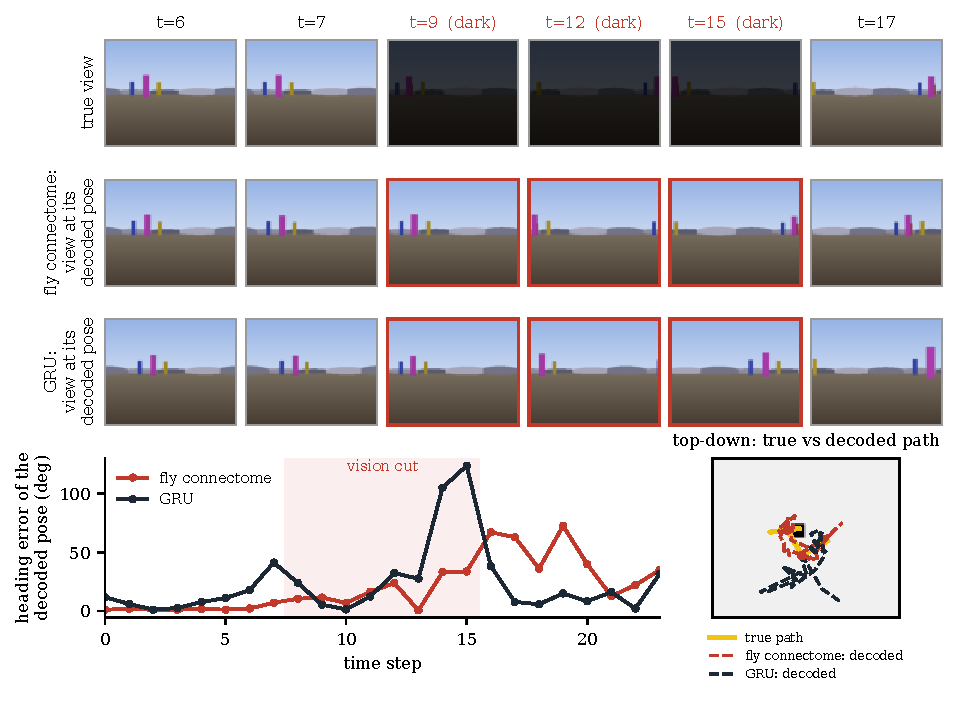
\includegraphics[width=\linewidth]{fig/video_strip.pdf}
  \caption{\textbf{What each network sees, thinks and decodes through a blackout} (one test episode, chosen as the one
  closest to the population medians for both models; video in the supplement). Top row: the panorama the teacher
  receives, dimmed during the vision cut. Middle rows: the arena rendered at the pose that a ridge readout decodes from
  each student's own activity at that moment, so each frame is literally where the network thinks it is. The connectome
  student's decoded view stays locked to the true view through the dark; the GRU's drifts. Bottom: heading error of the
  decoded pose over time, and the true path against both decoded paths. Both readouts show a transient when vision
  returns at $t{=}16$. The readout is fit on 400 training episodes and never sees this episode.}
  \label{fig:strip}
\end{figure*}

\paragraph{Seeing it} \cref{fig:strip} shows the effect on one episode: with vision cut, the pose read out of the
connectome state keeps rendering the right view, while the pose read out of the GRU state wanders. The interactive
version of this figure, with the live neuron state on the FlyWire coordinates, is in the supplement.

\paragraph{Dark duration} \cref{tab:dark} lengthens the window. Over 16 dark steps the connectome keeps heading
within \nConnArenaDarkSixteenHd\degree\ where the GRU is at \nGruArenaDarkSixteenHd\degree, and the real wiring's margin over
block-shuffled grows from \nConnBlockGapArena\degree\ to \nConnBlockGapArenaDarkSixteen\degree.

\subsection{Where the gap between sparse and dense models lives}
\label{sec:gap}

The attention-input rows of \cref{tab:pred,tab:probe} remove the one component the sparse students share with no
biological circuit: the 1.8\,M-parameter linear map from the fly-eye image into the VIS neurons. With a per-neuron
cross-attention encoder of 0.11\,M parameters, and the GRU and transformer re-matched to the smaller budget, the
sparse students predict at \nConnAttnArenaMse\ against \nGruAttnArenaMse\ (GRU) and \nTfAttnArenaMse\ (transformer),
and decode heading at \nConnAttnArenaHd\degree\ against \nGruAttnArenaHd\ and \nTfAttnArenaHd\degree. The prediction gap
therefore does not come from the input map, and the path-integration gap survives a better one.

The hybrid row asks the converse: what does the connectome lack? Adding one self-attention layer over the 796
cell-type-pooled activities to the recurrence (30\,k parameters, edge list unchanged) moves prediction to
\nHybridArenaMse\ and heading to \nHybridArenaHd\degree. \TODO{interpret once run 2 lands: does global routing close the
prediction gap, and does the code survive it?}

\subsection{Behaviour from the code}
\label{sec:behaviour}

\begin{figure*}[t]
  \centering
  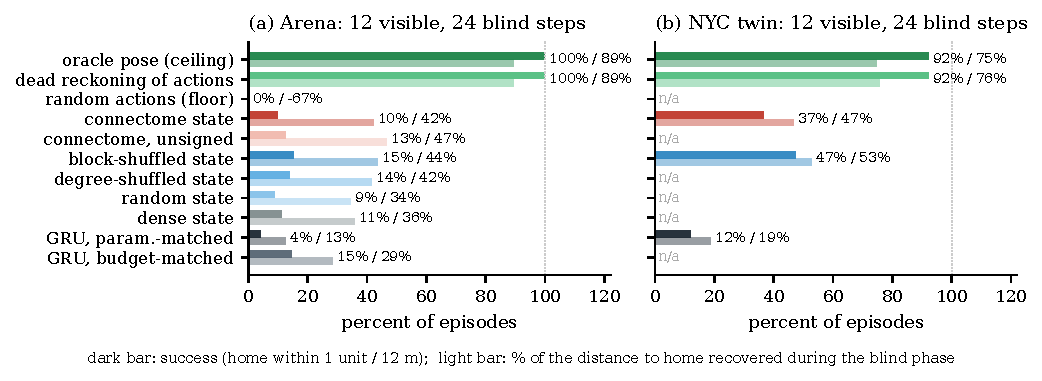
\includegraphics[width=\linewidth]{fig/homing.pdf}
  \caption{\textbf{Blind homing.} After 12 visible steps vision is cut and the same controller steers for 24 steps from
  one of several pose estimates. With the true pose or with dead reckoning of the action record it gets home almost
  every time, so the controller is not the limit. From a linear readout of a connectome-sized sparse state the agent
  recovers about half the distance; from the GRU or transformer state it barely moves. The real wiring has no edge over
  block-shuffled here.}
  \label{fig:homing}
\end{figure*}

\begin{table*}[t]
  \centering\small
  \setlength{\tabcolsep}{3.5pt}
  \begin{tabular}{lcccccc}
    \toprule
    & \multicolumn{2}{c}{Arena} & \multicolumn{2}{c}{Continuous turns} & \multicolumn{2}{c}{NYC twin} \\
    \cmidrule(lr){2-3}\cmidrule(lr){4-5}\cmidrule(lr){6-7}
    pose readout & \% closer & success & \% closer & success & \% closer & success \\
    \midrule
    oracle pose (controller ceiling) & 89 & 1.00 & -- & -- & 75 & 0.92 \\
    dead reckoning of actions & 89 & 1.00 & 87 & 0.90 & 76 & 0.92 \\
    random actions (floor) & -67 & 0.00 & -- & -- & -- & -- \\
    \midrule
    GRU, parameter-matched state & 13 & 0.04 & 21 & 0.16 & 19 & 0.12 \\
    GRU, recurrent-budget-matched state & 29 & 0.15 & -- & -- & -- & -- \\
    dense state & 36 & 0.11 & -- & -- & -- & -- \\
    connectome, unsigned state & \textbf{47} & 0.13 & -- & -- & -- & -- \\
    \textbf{connectome} state & 42 & 0.10 & \textbf{33} & \textbf{0.16} & 47 & 0.37 \\
    random state & 34 & 0.09 & -- & -- & -- & -- \\
    block-shuffled state & 44 & \textbf{0.15} & -- & -- & \textbf{53} & \textbf{0.47} \\
    degree-shuffled state & 42 & 0.14 & -- & -- & -- & -- \\
    \bottomrule
\end{tabular}

  \caption{\textbf{Blind homing from a linear readout of the state.} 12 visible then 24 blind steps; 50 test episodes
  per seed. \% closer is the reduction of the distance to home over the blind phase. On the continuous-turn arena the
  dead-reckoning controller is itself noisy. Every connectome-sized sparse student halves its distance from a linear
  readout; the GRU and transformer barely move. The real wiring has no edge over block-shuffled here.}
  \label{tab:homing}
\end{table*}

\cref{fig:homing} and \cref{tab:homing} ask whether the code is usable. The controller is not the bottleneck: with the
oracle pose or with dead reckoning of the action record it reaches home in almost every episode. From a linear readout
of the connectome state the agent recovers \nConnArenaCloser\,\% of its distance to home on the arena and
\nConnNycCloser\,\% on NYC, reaching it in \nConnNycSucc\ of NYC episodes, against \nGruNycSucc\ for the GRU and
\nTfNycSucc\ for the transformer. But arena success is only \nConnArenaSucc, and on NYC block-shuffled wiring does as
well or better. The behavioural effect is carried by connectome-scale sparse recurrence, not by synapse identity, and
the gap to the ceiling is the drift of a linear pose readout over 24 dark steps.

\paragraph{Goal-vector navigation (negative)} Steering toward a linearly decoded egocentric goal vector succeeds in
22\,\% of arena episodes for every wiring (GRU 22, random 21, dense 20) against 14\,\% for random actions and
92\,\% for the true goal vector; 5\,\% on NYC against 0 and 28. A 3- or 5-step vision cut changes nothing. The decoded
goal vector ($R^2$\,0.42 on closed-loop rollouts) is too coarse to steer with, and no wiring is better than another
(\cref{sec:suppl-goalnav}).

\subsection{Real handheld video}
\label{sec:realvid}

\begin{table*}[t]
  \centering\small
  \setlength{\tabcolsep}{4pt}
  \begin{tabular}{lcccccc}
    \toprule
    wiring & zero-shot MSE & fine-tuned MSE & heading, sim.\ readout & heading, clip readout & NYC model, zero-shot & NYC model, fine-tuned \\
    \midrule
    GRU, parameter-matched & 9.94\pm0.07 & \textbf{1.18\pm0.00} & 84.1\pm34.2 & 7.6\pm0.7 & \textbf{5.57\pm0.03} & -- \\
    dense & 9.73\pm0.07 & 1.21\pm0.04 & 29.5\pm6.4 & 9.1\pm0.9 & -- & -- \\
    connectome, unsigned & 9.59\pm0.13 & 1.26\pm0.00 & \textbf{24.3\pm6.3} & 7.7\pm0.3 & -- & -- \\
    \textbf{connectome} & 9.68\pm0.10 & 1.24\pm0.02 & 30.9\pm22.8 & 7.7\pm0.5 & 6.10\pm0.03 & -- \\
    random & \textbf{9.56\pm0.19} & 1.26\pm0.01 & 79.1\pm14.5 & 9.9\pm1.1 & 6.00\pm0.02 & -- \\
    degree-shuffled & 9.69\pm0.09 & 1.25\pm0.02 & 88.7\pm27.0 & \textbf{7.1\pm0.6} & 6.01\pm0.05 & -- \\
    \midrule
    copy last visible latent & 0.84 & 0.84 & -- & -- & 0.84 & 0.84 \\
    constant mean & 10.28 & 10.28 & -- & -- & 10.28 & 10.28 \\
    actions only (linear floor) & -- & -- & -- & 4.7 & -- & -- \\
    \bottomrule
\end{tabular}

  \caption{\textbf{Real phone video as the world.} \nRvClips\ clips, \nRvEpisodes\ episodes, blind window 8:16. Left:
  blind MSE of every arena-trained student zero-shot and after leave-one-clip-out fine-tuning (10 epochs), against the
  trivial predictors on the same episodes. Middle: median heading error of a ridge readout that was fit in the
  simulator and applied to the real state (transfer), and of one fit on the other clips (in-domain), against a linear
  readout of the estimated action record. Right: the same for the students trained on the NYC twin.}
  \label{tab:realvid}
\end{table*}

\begin{figure*}[t]
  \centering
  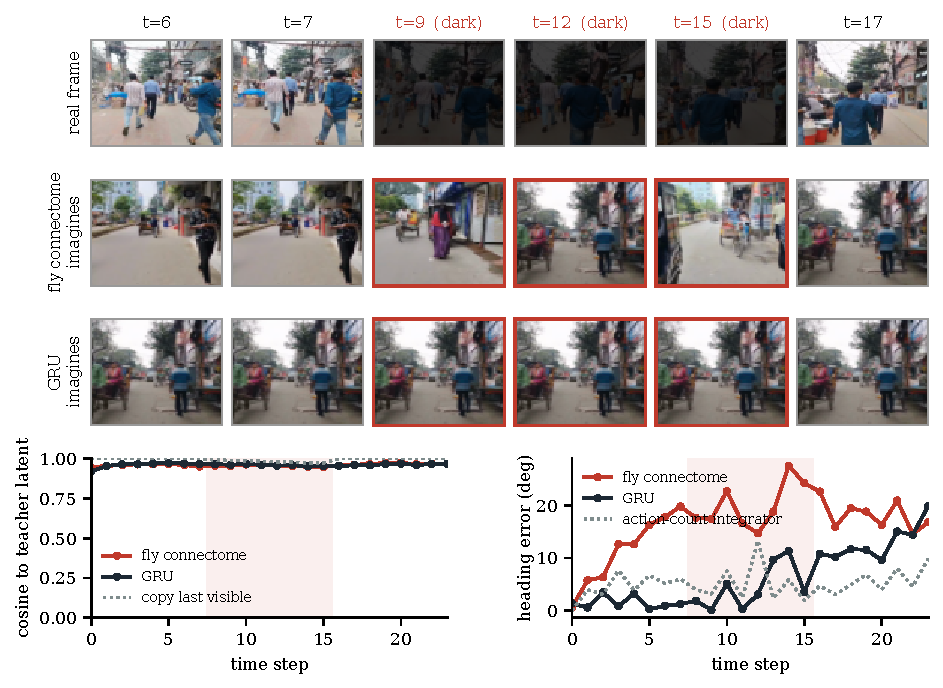
\includegraphics[width=\linewidth]{fig/realvid_strip.pdf}
  \caption{\textbf{The same test on real handheld video} (one held-out phone clip; both students fine-tuned on the
  other clips; video in the supplement). Top: the real frame, dimmed during the vision cut. Middle rows: the training
  frame whose teacher latent is nearest to each student's guess, \ie what each imagines. Bottom left: cosine to the
  teacher latent against a copy-last baseline (dotted). Bottom right: heading decoded from the state against the clip's
  own egomotion estimate, with a plain count of the estimated turn actions (dotted).}
  \label{fig:realvid}
\end{figure*}

\cref{tab:realvid} puts every architecture on the \nRvClips\ phone clips. Zero-shot every student is off distribution
(MSE \nConnRvMse\ for the connectome, \nGruRvMse\ for the GRU, against \nCopyLastRvMse\ for copy-last), and after
fine-tuning all reach about \nConnRvFtMse\ to \nGruRvFtMse, still above the copy-last baseline, because at 2\,Hz the
teacher latent of handheld footage changes little between steps. The heading probe is the informative part. With the
readout fit in the simulator and applied to the real state the connectome decodes the clip's egomotion to
\nConnRvTransferHd\degree\ against \nGruRvTransferHd\degree\ for the GRU; with a readout fit on the other clips the
numbers are \nConnRvIndomainHd\ and \nGruRvIndomainHd\degree\ against \nActOnlyRvHd\degree\ for a linear readout of the
estimated action record. \TODO{state the verdict once run 2 lands: does the simulator-fit heading code transfer to real
footage for the sparse students and not for the dense ones, as in the pilot, and is the in-domain probe above the
action-count floor?} Real video remains the weakest link of the paper: the footage has no odometry ground truth, the
egomotion estimate is itself a model, and the clips are short. We report it in full rather than drop it.

\subsection{Cost, data efficiency, scaling, ablation}
\label{sec:more}

\paragraph{Cost} At batch 1 one connectome step costs 7.4\,MFLOP, the same as the parameter-matched GRU, with 91,663
recurrent weights against the GRU's 580,644; the transformer costs more per step and grows with the context it
attends over; dense costs 103\,MFLOP. The sparse student is cheap in weights, not in wall-clock at this scale, where
every model is launch-bound.

\paragraph{Data efficiency} At 50, 100, 200 and 500 training episodes the ordering of \cref{tab:pred} is unchanged:
the GRU leads at every size and the connectome beats block-shuffled by 1 to 3\,\% (\cref{sec:suppl-data}). A prior
that should matter most with little data does not change the ranking.

\paragraph{Multi-brain scaling} Coupling $K=2$ or $3$ copies of the connectome through the real commissural edges gives
no gain (MSE 0.576, 0.577 vs 0.575 for $K=1$); the heading code is unchanged (7.0\degree, 8.7\degree\ vs 8.5\degree).

\paragraph{Subgraph ablation}
\label{sec:ablation}
With the synapse threshold at 1, 5 or 10, with the mushroom bodies or the descending neurons removed, or with the
central complex alone, the real wiring beats its degree-shuffled twin by 0.02 to 0.04 MSE (one seed each;
\cref{tab:ablation}). No single region carries the margin.
